\documentclass[aspectratio=169, table]{beamer}

%\usepackage[beamertheme=./praditatheme]{Pradita}
\usepackage[utf8]{inputenc}

\usetheme{Pradita}

\subtitle{MTI102-Information System \&\\Technology Architecture}

\title{Fase B: Arsitektur Bisnis dalam Metode Pengembangan Arsitektur TOGAF}
\date[Serial]{\scriptsize {PRU/SPMI/FR-BM-18/0222}}
\author[Pradita]{\small {\textbf{Alfa Yohannis}}}

\begin{document}

	\frame{\titlepage}

	\begin{frame}
		\frametitle{Tujuan}
		\begin{enumerate}
			\item Membangun Arsitektur Bisnis Target yang menjelaskan bagaimana perusahaan seharusnya beroperasi untuk mencapai tujuan bisnis, dan menaggapi penggerak bisnis strategis yang ditetapkan dalam Visi Arsitektur, dengan cara yang memenuhi atau menjawab \textit{Permintaan untuk Pekerjaan Arsitektur} dan \textit{hal-hal yang menjadi perhatian pemangku kepentingan}.

			\item Mengidentifikasi komponen Peta Jalan Arsitektur berdasarkan gap antara Arsitektur Saat Ini dan Arsitektur Bisnis Target.
		\end{enumerate}
	\end{frame}

	\begin{frame}
		\frametitle{Input (1)}
		\begin{columns}
			\begin{column}{0.5\textwidth}
				\begin{center}
					\begin{enumerate}

						\item Prinsip-prinsip Bisnis, tujuan bisnis, dan penggerak bisnis
						\item Penilaian Kapabilitas
						\item Rencana Komunikasi
						\item Model Organisasi untuk Arsitektur Perusahaan
						\item Kerangka Kerja Arsitektur yang Disesuaikan
						\item Pernyataan Kerja Arsitektur yang Disetujui

					\end{enumerate}
				\end{center}
			\end{column}
			\begin{column}{0.5\textwidth}
				\begin{center}
					\begin{enumerate}
						\setcounter{enumi}{7}
						\item Prinsip-prinsip Arsitektur, termasuk prinsip-prinsip bisnis yang sudah ada sebelumnya
						\item Kontinum Perusahaan
						\item Repositori Arsitektur
						\item Visi Arsitektur, termasuk:
						\begin{itemize}
							\item Permasalahan
							\item Tujuan Pernyataan Kerja Arsitektur
							\item Tinjauan ringkasan
							\item Skenario bisnis (opsional)
							\item Persyaratan pemangku kepentingan tingkat tinggi yang terperinci
						\end{itemize}

					\end{enumerate}
				\end{center}
			\end{column}
		\end{columns}
	\end{frame}

	\begin{frame}
		\frametitle{Input (2)}
		\begin{enumerate}
			\setcounter{enumi}{11}
			\item Rancangan Dokumen Definisi Arsitektur, termasuk (bila dalam cakupan):
			\begin{itemize}
				\item Arsitektur Bisnis Dasar (tingkat tinggi)
				\item Arsitektur Data Dasar (tingkat tinggi)
				\item Arsitektur Aplikasi Dasar (tingkat tinggi)
				\item Arsitektur Teknologi Dasar (tingkat tinggi)
				\item Arsitektur Bisnis Target (tingkat tinggi)
				\item Arsitektur Data Target (tingkat tinggi)
				\item Arsitektur Aplikasi Target (tingkat tinggi)
				\item Arsitektur Teknologi Target (tingkat tinggi)
			\end{itemize}
				\item Permintaan untuk Pekerjaan Arsitektur
		\end{enumerate}
	\end{frame}

	\begin{frame}
		\frametitle{Langkah-langkah}
		\begin{enumerate}
			\item Memilih model referensi, sudut pandang pelbagai aktor, dan alat-alat
			\item Mengembangkan Deskripsi Arsitektur Bisnis Saat Ini
			\item Mengembangkan Deskripsi Arsitektur Bisnis Target
			\item Melakukan Analisis Gap
			\item Mendefinisikan komponen-komponen peta jalan
		\end{enumerate}


	\end{frame}

	\begin{frame}
		\frametitle{Langkah-langkah(2)}
		\begin{enumerate}
			\setcounter{enumi}{5}
			\item Membuat solusi atas dampak/efek samping di seluruh Lanskap Arsitektur
			\item Melakukan kajian pemangku kepentingan secara formal terhadap arsitektur yang diajukan.
			\item Menyelesaikan Arsitektur Bisnis
			\item Membuat Dokumen Definisi Arsitektur
		\end{enumerate}


	\end{frame}


	\begin{frame}
		\frametitle{Output}
		\begin{enumerate}
			\item Pernyataan Kerja Arsitektur, diperbarui jika diperlukan
			\item Prinsip-prinsip bisnis yang tervalidasi, tujuan bisnis, dan penggerak bisnis
			\item Prinsip-prinsip Arsitektur Bisnis yang dimuktahirkan
			\item Draf Dokumen Definisi Arsitektur, termasuk konten yang telah diperbaharui
			\item Draf Spesifikasi Persyaratan Arsitektur, termasuk konten yang telah diperbaharui
			\item Komponen Arsitektur Bisnis dari Peta Jalan Arsitektur
		\end{enumerate}
	\end{frame}

	\begin{frame}
		\frametitle{Menggunakan Repositori Arsitektur}
		\framesubtitle{\hspace{1cm}}
		Tim arsitektur perlu mempertimbangkan sumber daya Arsitektur Bisnis yang relevan yang tersedia dari Repositori Arsitektur, terutama:
		\begin{enumerate}
			\item standar umum yang berlaku
			\item Model bisnis generik yang relevan dengan sektor industri organisasi (industri ritel dan kesehatan)
			\item Model bisnis yang relevan dengan domain bisnis (ritel alat kesehatan)
			\item Blok bangunan khusus perusahaan (komponen proses, aturan bisnis, deskripsi pekerjaan, dll.)

		\end{enumerate}
	\end{frame}


	\begin{frame}
		\frametitle{Mengidenfikasi Katalog, Matrix, dan Diagram}
		\framesubtitle{\hspace{1cm}}
		\begin{enumerate}
			\item Katalog mengumpulkan inventaris aset inti bisnis.
			\item Matriks menunjukkan hubungan inti antara entitas model.
			\item Diagram menggambarkan informasi Arsitektur Bisnis dari berbagai perspektif (pandangan).
		\end{enumerate}
	\end{frame}

	{
		\setbeamertemplate{navigation symbols}{}
		\setbeamertemplate{footline}{}
		\begin{frame}
			\centering
			\frametitle{Katalog, Matrix, dan Diagram}
			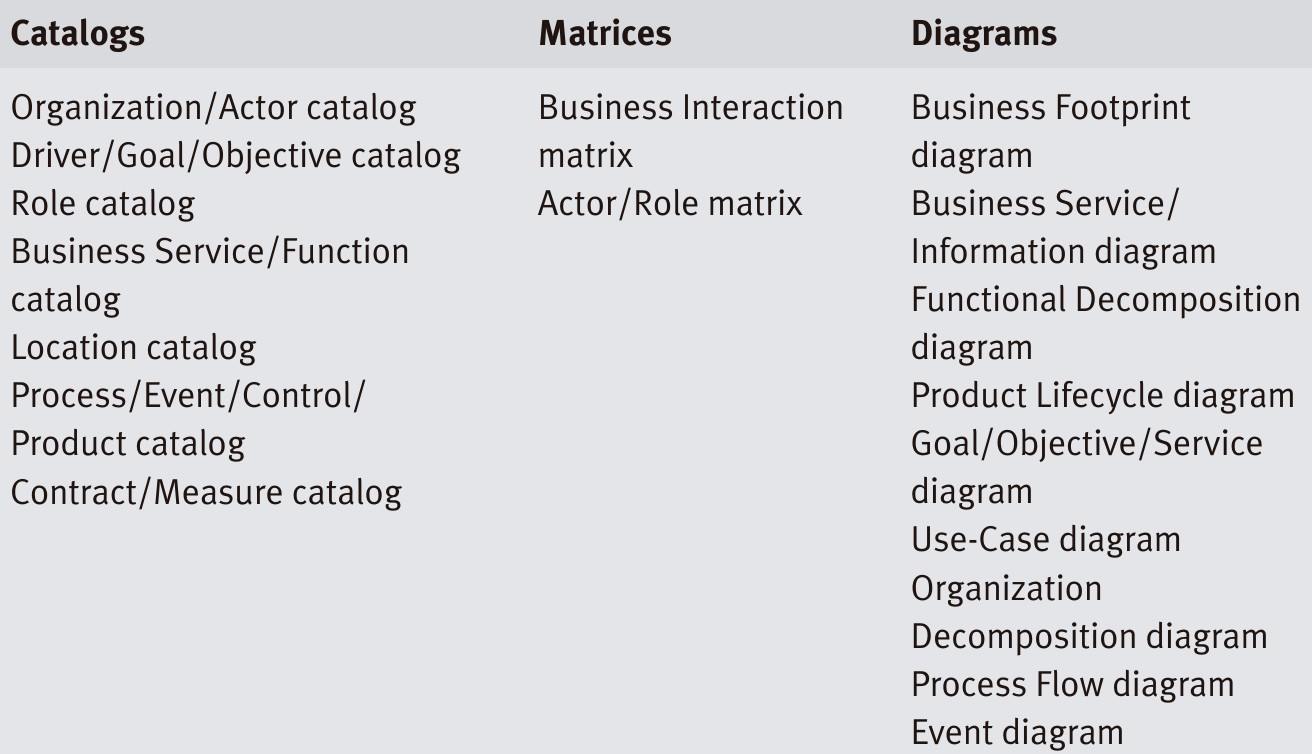
\includegraphics[width=.6\textwidth]{../figures/catalogs_matrices_diagrams.png}
		\end{frame}
	}

	\begin{frame}
		\frametitle{Isi Dokumen Definisi Arsitektur}
%		\framesubtitle{\hspace{1cm}}
		\begin{columns}
			\begin{column}{0.5\textwidth}
				\begin{center}
					\begin{enumerate}
						\item Lingkup
						\item Tujuan, objektif, dan kendala
						\item Prinsip-prinsip arsitektur
						\item Arsitektur dasar
						\item Model arsitektur (untuk setiap keadaan yang akan dimodelkan); seperti model untuk Arsitektur Bisnis, Arsitektur Data, Arsitektur Aplikasi, dan Arsitektur Teknologi

					\end{enumerate}
				\end{center}
			\end{column}
			\begin{column}{0.5\textwidth}
				\begin{center}
					\begin{enumerate}
						\setcounter{enumi}{5}
						\item Rationale dan justifikasi untuk pendekatan arsitektur
						\item Pemetaan ke Repositori Arsitektur, termasuk pemetaan ke Lanskap Arsitektur, model referensi, standar, serta penilaian penggunaan kembali
						\item Analisis kesenjangan
						\item Penilaian dampak
						\item Arsitektur Transisi
					\end{enumerate}
				\end{center}
			\end{column}
		\end{columns}
	\end{frame}

	\begin{frame}
		\frametitle{Isi Komponen Arsitektur Bisnis}
		\begin{enumerate}
			\item Baseline Arsitektur Bisnis, jika sesuai; ini adalah deskripsi dari Arsitektur Bisnis yang ada.
			\item Target Arsitektur Bisnis, termasuk:
			\item Tampilan yang sesuai dengan pandangan yang dipilih untuk mengatasi kekhawatiran pemangku kepentingan utama.
		\end{enumerate}
	\end{frame}

		\begin{frame}
		\frametitle{Isi Komponen Arsitektur Bisnis(2)}
%		\framesubtitle{\hspace{1cm}}
		\begin{enumerate}
			\setcounter{enumi}{3}
			\item Target Arsitektur Bisnis, termasuk:
			\begin{itemize}
				\item \textbf{Struktur organisasi} yang mengidentifikasi lokasi bisnis dan menghubungkannya dengan unit organisasi.
				\item \textbf{Tujuan dan objektif bisnis} untuk perusahaan dan setiap unit organisasi.
				\item \textbf{Fungsi bisnis} yang diidentifikasi menggunakan langkah rinci dan rekursif yang melibatkan dekomposisi berurutan dari area fungsi utama menjadi sub-fungsi.
				\item \textbf{Layanan bisnis} yang diberikan oleh perusahaan dan setiap unit perusahaan kepada pelanggannya, baik internal maupun eksternal.
			\end{itemize}
		\end{enumerate}
	\end{frame}


	\begin{frame}
		\frametitle{Isi Komponen Arsitektur Bisnis (3)}
%		\framesubtitle{\hspace{1cm}}
			\begin{itemize}
                \item \textbf{Proses bisnis}, termasuk ukuran dan hasil yang dihasilkan.
				\item \textbf{Peran bisnis}, termasuk pengembangan dan modifikasi persyaratan keahlian.
				\item \textbf{Model data bisnis}.
				\item \textbf{Korelasi organisasi dan fungsi} yang menghubungkan fungsi bisnis dengan unit organisasi dalam bentuk laporan matriks.
			\end{itemize}
	\end{frame}



	\begin{frame}
		\frametitle{Isi Spesifikasi Kebutuhan Arsitektur}
		\framesubtitle{\hspace{1cm}}
		\begin{columns}
			\begin{column}{0.5\textwidth}
				\begin{center}
					\begin{enumerate}
						\item Ukuran keberhasilan
						\item Persyaratan arsitektur
						\item Kontrak layanan bisnis
						\item Kontrak layanan aplikasi
						\item Panduan implementasi
						\item Spesifikasi implementasi

					\end{enumerate}
				\end{center}
			\end{column}
			\begin{column}{0.5\textwidth}
				\begin{center}
					\begin{enumerate}
						\setcounter{enumi}{6}
						\item Standar implementasi
						\item Persyaratan interoperabilitas
						\item Persyaratan manajemen layanan TI
						\item Kendala
						\item Asumsi
					\end{enumerate}
				\end{center}
			\end{column}
		\end{columns}
	\end{frame}

	\begin{frame}
		\frametitle{Kebutuhan Arsitektur Bisnis}
%		\framesubtitle{\hspace{1cm}}
		\begin{enumerate}
			\item Hasil Analisis Gap
			\item Kebutuhan bisnis yang diperbarui, diidentifikasi dengan menggunakan teknik Skenario Bisnis
		\end{enumerate}
	\end{frame}

	\begin{frame}
		\frametitle{Kebutuhan Arsitektur Bisnis (2)}
%		\framesubtitle{\hspace{1cm}}
		\begin{enumerate}
			\setcounter{enumi}{2}
			\item Kebutuhan teknis: Sebuah set awal kebutuhan teknis harus dihasilkan sebagai output dari Fase B: Arsitektur Bisnis. Ini menjadi pendorong untuk pekerjaan Arsitektur Teknologi yang akan datang, dan harus mengidentifikasi, mengategorikan, dan mengutamakan implikasi untuk pekerjaan di domain arsitektur yang tersisa; misalnya, dengan menggunakan matriks ketergantungan/prioritas (misalnya, memandu kompromi antara kecepatan pemrosesan transaksi dan keamanan) dan daftar model khusus yang diharapkan dihasilkan.

		\end{enumerate}
	\end{frame}


	\begin{frame}
		\frametitle{Ringkasan}
%		\framesubtitle{\hspace{1cm}}
		\begin{enumerate}
			\item Fase Arsitektur Bisnis memungkinkan kita untuk mendefinisikan dan memvalidasi arsitektur bisnis yang diperlukan untuk mendukung strategi bisnis.
			\item Fase ini penting untuk memastikan bahwa arsitektur bisnis sejalan dengan kebutuhan stakeholder.
		\end{enumerate}
	\end{frame}

\end{document}
